\begin{frame}
\frametitle{Qubit}
\begin{columns}
  \begin{column}{0.5\textwidth}
    \begin{figure}
      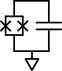
\includegraphics[scale=1.8]{transmon.pdf}
      \caption*{Transmon qubit}
    \end{figure}
  \end{column}
  \begin{column}{0.5\textwidth}
    \begin{figure}
      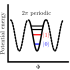
\includegraphics[scale=2.2]{cosine_potential.pdf}
    \end{figure}
  \end{column}
\end{columns}
\begin{columns}
  \begin{column}{0.5\textwidth}
    \begin{itemize}
      \item Josephson junction (cross): nonlinear inductor
      \item $H_\text{junction} = - E_J \cos(2\pi \Phi / \Phi_0)$
    \end{itemize}
  \end{column}
  \begin{column}{0.5\textwidth}
    \begin{itemize}
      \item Cosine potential from junction
      \item Unevenly spaced levels
      \item Bottom two levels form qubit
    \end{itemize}
  \end{column}
\end{columns}
\end{frame}
